% !TEX TS-program = pdflatex

\documentclass[unicode,11pt,notheorems,xcolor=table]{beamer}

\usepackage[T2A]{fontenc}
\usepackage[utf8]{inputenc}
\usepackage[russian]{babel}
\usepackage{amsmath,amsfonts,amssymb,amsthm}
\usepackage{mathtools}
\usepackage{diagbox}

\usepackage{ulem}
\usepackage{tikz, graphicx}
%\usepackage{tkz-graph}
\usetikzlibrary{matrix,arrows,decorations.pathmorphing, arrows.meta,positioning}
\usetikzlibrary{positioning,calc}
\usetikzlibrary{petri}
\usetikzlibrary{decorations.pathreplacing}

%Описание стиля презентации
\usetheme[sidebar=0]{kfmn} 
\setbeamercovered{transparent}

%\definecolor{cyan}{RGB}{240,217,1}
%\definecolor{vgugreen}{RGB}{143,188,103}
%\definecolor{vgured}{RGB}{234,38,40}
%\definecolor{vgublue}{RGB}{53,101,167}



\makeatletter
	\g@addto@macro{\endtabular}{\rowfont{}}% Clear row font
	\makeatother
	\newcommand{\rowfonttype}{}% Current row font
	\newcommand{\rowfont}[1]{% Set current row font
		\gdef\rowfonttype{#1}#1\ignorespaces%
	}
\makeatother

\newcommand{\myunit}{9mm}
\tikzset{
    node style sp/.style={draw,circle,minimum size=\myunit},
    node style ge/.style={circle,minimum size=\myunit},
    arrow style mul/.style={draw,sloped,midway,fill=white},
    arrow style plus/.style={midway,sloped,fill=white},
}

%[0, 6, 8, 8, 10, 5, 6, 10, 8, 10, 10], 

\pgfdeclareimage[height=8mm]{university-logo}{logo-iem.png}
\logo{\pgfuseimage{university-logo}}
%2[0, 11, 10, 8, 11, 5, 11, 11, 8, 11, 10, 11],

\titlepicture{
	\begin{tikzpicture}[y=1.4cm,overlay,rotate=8]
	\coordinate (O) at (-3cm,0.9cm);
	\filldraw[thick,draw= vgublue, fill=vgublue!20!white] (0,0) circle[radius=4.2cm];
	\clip (0,0) circle[radius=4.2cm];
	\draw (-1.5,1.5) node{
	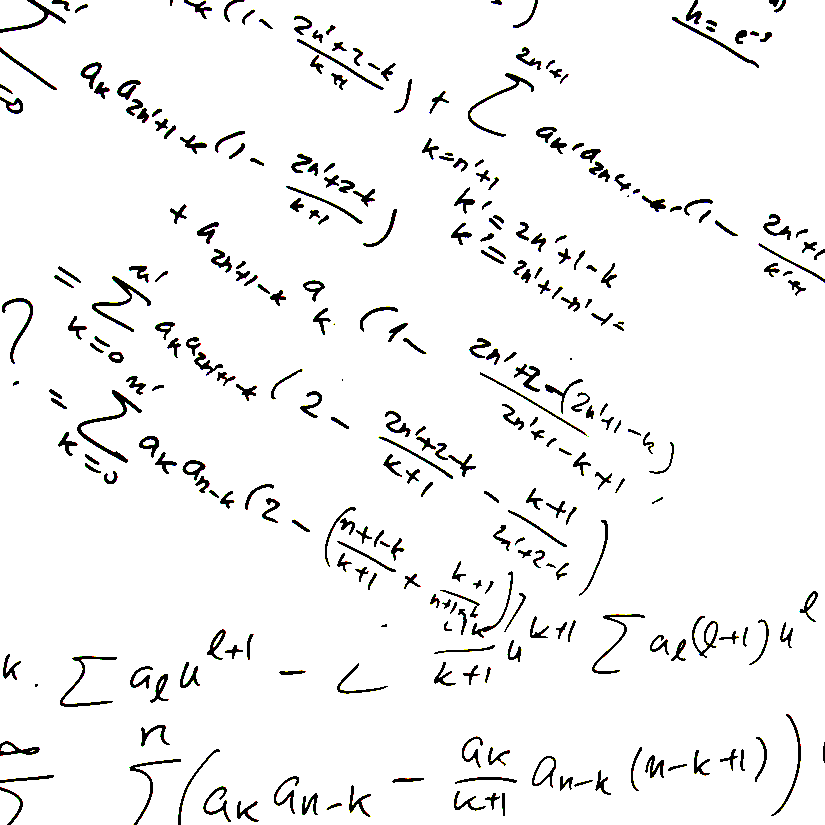
\includegraphics[width=8cm]{titlepic.png}
	};
\end{tikzpicture}
}

\usepackage[math]{iwona}

\newcommand{\hplus}{\mathbin{\hat+}}
\newcommand{\hdot}{\mathbin{\hat\cdot}}
% Описание теорем
\newtheorem{theorem}{Теорема}
\newtheorem{seq}{Следствие}
%%

\LECT % 

% Титульный лист теорем
\author[Д.\,В. Чупраков]{канд.\,физ.-матем.\,наук, доцент Д.\,В. Чупраков\\[6pt] usr10381@vyatsu.ru}

\institute[ВятГУ]{ФГБОУ ВО Вятский государственный университет}

\department{Факультет экономики и финансов}

\title[Лекция~10. Многокритериальные задачи]{
	Введение в экономико-математическое моделирование\\[12pt]
	Лекция~10. Многокритериальные задачи}

\date{2 ноября 2020~г.}


\setbeamercovered{invisible}



\begin{document}


\maketitle

\begin{frame}{Структура лекции}
	\tableofcontents
\end{frame}

\section{Проблема нескольких критериев}

\begin{frame}{Проблемы многокритериальной оптимизации}{}
\begin{enumerate}
    \item Проблема нормализации критериев, то  есть приведение критериев к единому масштабу измерения.
    \item Проблема выбора принципа оптимальности, то есть установление, в каком смысле оптимальное решение лучше всех остальных решений.
    \item Проблема учета приоритетов критериев, возникающая в тех случаях, когда из экономического смысла критериев ясно, что некоторые из них имеют приоритет над другими. 
    \item Проблема выбора метода вычисления оптимума задачи. 
\end{enumerate}
\begin{alertblock}{}
    Многокритериальная задача может не иметь оптимального решения.
\end{alertblock}
\end{frame}

 \section{Каноническая двукритериальная задача оптимизации}


\begin{frame}{Задача многокритериальной оптимизации}
    \begin{itemize}
        \item Имеется область допустимых планов.
        \item Есть несколько целевых функций.
        \item Целевые функции не могут быть совмещены в одну.
    \end{itemize}
    \medskip
    \hrule
    \medskip
    Требуется найти точку области допустимых решений, в которой достигается максимум (или минимум) всех целевых функций. 

    \medskip
    \hrule
    \medskip
    \alert{Важно:}
    В оптимальном плане многокритериальной задачи каждый критерий в отдельности может не достигать своего оптимума.

\end{frame}

\begin{frame}{Каноническая двукритериальная задача оптимизации}{}
    \begin{itemize}
        \item Каждый из критериев максимизируется:
        $$
            F_1(x_1,x_2) \to \max, \qquad F_2(x_1,x_2) \to \max
        $$
        \item Область допустимых планов задана системой ограничений в форме нестрогих неравенств.
        $$  \left\lbrace
            \begin{aligned}
                h_1(x_1,x_2) \leqslant b_1\\
                h_2(x_1,x_2) \leqslant b_2\\
                &\cdots \\
                h_n(x_1,x_2) \leqslant b_n\\
            \end{aligned}
            \right.
        $$
        \end{itemize}
\end{frame}

\begin{frame}{Сведение задачи к канонической форме}{}
    Задача может быть поставлена по разному:

    \begin{itemize}
        \item $ F_1(x_1,x_2) \to \max, \qquad F_2(x_1,x_2) \to \max $
        \item $ F_1(x_1,x_2) \to \alert{\min}, \qquad F_2(x_1,x_2) \to \max $
        \item $ F_1(x_1,x_2) \to \alert{\min}, \qquad F_2(x_1,x_2) \to \alert{\min} $
    \end{itemize}
    \pause
    \begin{block}{}
        $$
        F(x_1,x_2) \to \min \Longleftrightarrow \alert{G(x_1,x_2)= -F(x_1,x_2)} \to \max
        $$
    \end{block}

    \bigskip
    Если критерий минимизируется, то нужно умножить его на $-1$.
\end{frame}

\section{Множество Парето}

\begin{frame}{Типы точек системы ограничений}
  
    {\centering
    \begin{tikzpicture}[>=latex,x=2.5mm,y=1.2mm]
        % \draw[dashed,thin,black!50] (0,0) grid (30,45);
        \draw[->](0,0) -- (30,0) node[right]{$F_2$};
        \draw[->](0,0) -- (0,45) node[left]{$F_1$};
        \fill[vgublue]
            (4,41) 
            coordinate (1) 
            % circle[radius=1.5pt]
            % node[right]{\scriptsize 1}
            
            (20,25) 
            coordinate (5) 
            circle[radius=1.5pt]
            node[right]{\scriptsize $B$}
            (25,0) 
            coordinate (30) 
            % circle[radius=1.5pt]
            % node[right]{\scriptsize 30}
            (10,10) 
            coordinate (A) 
             circle[radius=1.5pt]
             node[right]{\scriptsize $A$}

             (2.1,15) 
             coordinate (C) 
              circle[radius=1.5pt]
              node[left]{\scriptsize $C$}
 
            (18.85,14) 
              coordinate (D) 
               circle[radius=1.5pt]
               node[right]{\scriptsize $D$}
  
              ;
              
            \filldraw[fill=vgublue, fill opacity=0.3, draw=vgublue,thick]
            (1) .. controls +(3,-15) .. (5) .. controls +(-2,-15) .. (30)
            .. controls +(-25,+3) .. (1)
            ;            
            
            \fill[fill=vgured, fill opacity=0.5] (5) circle[radius=5mm];


            \fill[fill=vgured, fill opacity=0.5] (A) circle[radius=5mm];

            \fill[fill=vgured, fill opacity=0.5] (C) circle[radius=5mm];

            \fill[fill=vgured, fill opacity=0.5] (D) circle[radius=5mm];

    \end{tikzpicture}\par}
    \begin{itemize}
        \item \alert{$A$}~--- внутренняя точка;
        \item \alert{$B$}~--- вершинная точка;
        \item \alert{$C$}, \alert{$D$}~--- граничные точки.
    \end{itemize}
\end{frame}
\begin{frame}{Оптимальность по Парето}
   
\end{frame}

\begin{frame}{Лучший план по Парето}
    \begin{block}{Определеине}
        \alert{План $A(x_1,x_2)$ лучше плана $B_(y_1,y_2)$ по Парето} ($A \succcurlyeq Y$), если 
        $$
         F_1(x_1,x_2) \geqslant F_1(y_1,y_2), \qquad F_2(x_1,x_2) \geqslant F_2(y_1,y_2) \qquad 
         $$
    \end{block}

    \bigskip
    ,,Всякое изменение, которое никому не приносит убытков, а~некоторым людям приносит пользу (по их собственной оценке), является улучшением``
    
    {\raggedleft \small Вильфредо Парето\\ (15 июля 1848 -- 20 августа 1923)\\ 
    итальянский  инженер, экономист и социолог\par}
\end{frame}

\begin{frame}{Множество Парето}

    План $A$~--- \alert{Парето-оптимальный решение}, если не существует такого плана $B$, что $B \succcurlyeq A$ по Парето.
    
    \bigskip
    \begin{block}{}
        \alert{Множество Парето}~--- множество  всех Парето-оптимальных решений задачи.
    \end{block}
    \bigskip

  
    Итак, \alert{множество Парето}~--- это множество допустимых планов  в~задаче многокритериальной оптимизации, для которых не существует другого допустимого плана, имеющей по всем критериям не худшие оценки и хотя бы по одному критерию~--- лучшие.
        

    
\end{frame}

% \begin{frame}{Выбор Парето-оптимальных альтернатив при решении многокритериальной задачи}

% \end{frame}

\begin{frame}{Пример}{}
    \begin{exampleblock}{}
        Приближенно построить множество Парето для следующей задачи двухкритериальной оптимизации:
    
    $$  
    \begin{aligned}
        F_1 &= (x-2)^2+(y-1)^2 \to \max\\
        F_2 &= -(x-5)^2 -(y-5)^2 \to \min\\
    \end{aligned}
        \qquad
        D_X\colon 
        \left\lbrace
        \begin{aligned}
            0 \leqslant &x \leqslant 5\\
            1 \leqslant &y \leqslant 5    
        \end{aligned}
        \right.
    $$
\end{exampleblock}
\pause
Преобразуем задачу:

$$  
\begin{aligned}
    G_1 &= F_1 = (x-2)^2+(y-1)^2 \to \max\\
    G_2 &= -F_2 = (x-5)^2 + (y-5)^2 \to \max\\
\end{aligned}
    \qquad
    D_X\colon 
    \left\lbrace
    \begin{aligned}
        0 \leqslant &x \leqslant 5\\
        1 \leqslant &y \leqslant 5    
    \end{aligned}
    \right.
$$

\end{frame}

\begin{frame}{Пример. Cетка.}
    Покроем множество допустимых значений сеткой с шагом~1:
    
    {\centering
    \begin{tikzpicture}[>=latex]
        \draw[dashed] (0,0) grid (6,6);
        \draw[thick,->](0,0) -- (6.5,0) node[right]{$x$};
        \draw[thick,->](0,0) -- (0,6.5) node[left]{$y$};
        \filldraw[very thick, draw=vgublue, fill=vgublue, fill opacity=0.2](0,1) rectangle (5,5);
        \foreach \x in {0,...,5}
            \foreach \y in {1,...,5}
            {
                \pgfmathtruncatemacro{\lbl}{5*\x +\y};
                \node[
                    circle,
                    draw=black,
                    fill=vgured!40,
                     minimum size=2
                    ]
                    (\lbl) at (\x, \y) {\tiny \phantom{;}};
                \node[]
                    () at (\x, \y) {\scriptsize\lbl};
    
            }
    \end{tikzpicture}\par}
\end{frame}

\begin{frame}{Пример. Вычисление критериев в узлах}
\begin{tabular}{|c|c|c|c|c|c|c|}
    \hline
    \slashbox{$y$}{$x$} & 0& 1& 2& 3 & 4  & 5 \\
    \hline
    1 & \slashbox{4}{41} & \slashbox{1}{32} & \slashbox{0}{25} & \slashbox{1}{20} & \slashbox{4}{17}  & \slashbox{9}{16} \\
    \hline
    2 & \slashbox{5}{34} & \slashbox{2}{25} & \slashbox{1}{18} & \slashbox{2}{13} & \slashbox{5}{10}  & \slashbox{10}{~9} \\
    \hline
    3 & \slashbox{8}{29} & \slashbox{5}{20} & \slashbox{4}{13} & \slashbox{5~}{~~8} & \slashbox{8~~}{~5}  & \slashbox{13}{~4} \\
    \hline
    4 & \slashbox{13}{26} & \slashbox{10}{17} & \slashbox{9}{10} & \slashbox{10}{~5} & \slashbox{13}{~2}  & \slashbox{18}{~1} \\
    \hline
    5 & \slashbox{20}{25} & \slashbox{17}{16} & \slashbox{16}{9} & \slashbox{17}{~4} & \slashbox{20}{~1}  & \slashbox{25}{~0} \\
    \hline
\end{tabular}
\begin{itemize}
    \item \structure{cверху слева} $G_1 = (x-2)^2+(y-1)^2$
    \item \structure{снизу справа} $G_2 = (x-5)^2+(y-5)^2$
\end{itemize}
\end{frame}

\begin{frame}{Пример. Множество достижимых значений $G$}
  
    {\centering
    \begin{tikzpicture}[>=latex,x=2.5mm,y=1.6mm]
        \draw[dashed,thin,black!50] (0,0) grid (30,45);
        \draw[->](0,0) -- (30,0) node[right]{$G_1$};
        \draw[->](0,0) -- (0,45) node[left]{$G_2$};
        \fill[vgublue]
            (4,41) 
            coordinate (1) 
            circle[radius=1.5pt]
            node[right]{\scriptsize 1}
            
            (5,34) 
            coordinate (2) 
            circle[radius=1.5pt]
            node[right]{\scriptsize 2}

            (8,29) 
            coordinate (3) 
            circle[radius=1.5pt]
            node[right]{\scriptsize 3}

            (13,26) 
            coordinate (4) 
            circle[radius=1.5pt]
            node[right]{\scriptsize 4}

            (20,25) 
            coordinate (5) 
            circle[radius=1.5pt]
            node[right]{\scriptsize 5}
            %----
            (1,32) 
            coordinate (6) 
            circle[radius=1.5pt]
            node[right]{\scriptsize 6}
            
            (2,25) 
            coordinate (7) 
            circle[radius=1.5pt]
            node[right]{\scriptsize 7}

            (5,20) 
            coordinate (8) 
            circle[radius=1.5pt]
            node[right]{\scriptsize 8}

            (10,17) 
            coordinate (9) 
            circle[radius=1.5pt]
            node[right]{\scriptsize 9}

            (17,16) 
            coordinate (10) 
            circle[radius=1.5pt]
            node[right]{\scriptsize 10}
            %----
            (0,25) 
            coordinate (11) 
            circle[radius=1.5pt]
            node[right]{\scriptsize 11}
            
            (1,18) 
            coordinate (12) 
            circle[radius=1.5pt]
            node[right]{\scriptsize 12}

            (4,13) 
            coordinate (13) 
            circle[radius=1.5pt]
            node[right]{\scriptsize 13}

            (9,10) 
            coordinate (14) 
            circle[radius=1.5pt]
            node[right]{\scriptsize 14}

            (16,9) 
            coordinate (15) 
            circle[radius=1.5pt]
            node[right]{\scriptsize 15}
            
            
            %----
            (1,20) 
            coordinate (16) 
            circle[radius=1.5pt]
            node[right]{\scriptsize 16}
            
            (2,13) 
            coordinate (17) 
            circle[radius=1.5pt]
            node[right]{\scriptsize 17}

            (5,8) 
            coordinate (18) 
            circle[radius=1.5pt]
            node[right]{\scriptsize 18}

            (10,5) 
            coordinate (19) 
            circle[radius=1.5pt]
            node[right]{\scriptsize 19}

            (17,4) 
            coordinate (20) 
            circle[radius=1.5pt]
            node[right]{\scriptsize 20}            
            
            %----
            (4,17) 
            coordinate (21) 
            circle[radius=1.5pt]
            node[right]{\scriptsize 21}
            
            (5,10) 
            coordinate (22) 
            circle[radius=1.5pt]
            node[right]{\scriptsize 22}

            (8,5) 
            coordinate (23) 
            circle[radius=1.5pt]
            node[right]{\scriptsize 23}

            (13,2) 
            coordinate (24) 
            circle[radius=1.5pt]
            node[right]{\scriptsize 24}

            (20,1) 
            coordinate (25) 
            circle[radius=1.5pt]
            node[right]{\scriptsize 25}
           %----
           (9,16) 
           coordinate (26) 
           circle[radius=1.5pt]
           node[right]{\scriptsize 26}
           
           (10,9) 
           coordinate (27) 
           circle[radius=1.5pt]
           node[right]{\scriptsize 27}

           (13,4) 
           coordinate (28) 
           circle[radius=1.5pt]
           node[right]{\scriptsize 28}

           (18,1) 
           coordinate (29) 
           circle[radius=1.5pt]
           node[right]{\scriptsize 29}

           (25,0) 
           coordinate (30) 
           circle[radius=1.5pt]
           node[right]{\scriptsize 30}
        ;
        \draw 
            (11)--(6)--(1)--(2)--(3)--(4)--(5)--
            (10)--(15)--(20)--(25)--(30)
            (11)--(12)--(17)--(18)--(23)--(24)--(29)--(30);            


        \draw[very thick, vgured]
            (1)--(2)--(3)--(4)--(5)
            (25)--(30);
        
        \fill [ vgured]
            (1) circle[radius=2pt]
            (2) circle[radius=2pt]
            (3) circle[radius=2pt]
            (4) circle[radius=2pt]
            (5) circle[radius=2pt]
            (30) circle[radius=2pt];
        \fill [vgublue]
            (25) circle[radius=2pt];


    \end{tikzpicture}\par}
\end{frame}

\begin{frame}{Множество Парето}
    
    {\centering
    \begin{tikzpicture}[>=latex]
        \draw[dashed] (0,0) grid (6,6);
        \draw[thick,->](0,0) -- (6.5,0) node[right]{$x$};
        \draw[thick,->](0,0) -- (0,6.5) node[left]{$y$};
        \filldraw[very thick, draw=vgublue, fill=vgublue, fill opacity=0.2](0,1) rectangle (5,5);
        \foreach \x in {0,...,5}
            \foreach \y in {1,...,5}
            {
                \pgfmathtruncatemacro{\lbl}{5*\x +\y};
                \node[
                    circle,
                    draw=black,
                    fill=white,
                     minimum size=2
                    ]
                    (\lbl) at (\x, \y) {\tiny \phantom{;}};
            }

            % \draw[very thick]
            %     (11) -- (12) -- (18) -- (24) -- (30)--(23) -- (17) -- (11);
            % \node[circle,fill=vgured!50]
            %     () at (11) {\tiny \phantom{;}};
            % \node[circle,fill=vgured!50]
            %     () at (12) {\tiny \phantom{;}};
            % \node[circle,fill=vgured!50]
            %     () at (18) {\tiny \phantom{;}};
            % \node[circle,fill=vgured!50]
            %     () at (24) {\tiny \phantom{;}};
            % \node[circle,fill=vgured!50]
            %     () at (30) {\tiny \phantom{;}};
            % \node[circle,fill=vgured!50]
            %     () at (23) {\tiny \phantom{;}};
            % \node[circle,fill=vgured!50]
            %     () at (17) {\tiny \phantom{;}};


            \draw[line width= 6pt, draw opacity = 0.5,vgured]
                (1) -- (2) -- (3) -- (4) -- (5)
                (25) -- (30);
            \node[circle,fill=vgured!50]
                () at (1) {\tiny \phantom{;}};
            \node[circle,fill=vgured!50]
                () at (2) {\tiny \phantom{;}};
            \node[circle,fill=vgured!50]
                () at (3) {\tiny \phantom{;}};
            \node[circle,fill=vgured!50]
                () at (4) {\tiny \phantom{;}};
            \node[circle,fill=vgured!50]
                () at (5) {\tiny \phantom{;}};
            \node[circle,fill=vgured!50]
                () at (30) {\tiny \phantom{;}};

        \foreach \x in {0,...,5}
            \foreach \y in {1,...,5}
            {
                \pgfmathtruncatemacro{\lbl}{5*\x +\y};
                \node[]
                    () at (\x, \y) {\scriptsize\lbl};
    
            }
            
    \end{tikzpicture}\par}
\end{frame}



\begin{frame}{Алгоритм построения множества Парето }{}
    \structure{Пусть дана задача с двумя переменными и двумя критериями}

    \begin{enumerate}
        \item Построить систему ограничений.
        \item Выбрать шаг сетки и отметить узлы этой сетки, лежащие внутри области допустимых планов.
        \item Посчитать значение критериев $F_1,F_2$ в каждом узле. Отметить соответствующие точки в системе координат $OF_1F_2$.
        \item Для задачи минимума отметить все точки такие, что ниже и левее них нет точек, соответствующих другим узлам сетки.
         \item Для задачи максимума отметить все точки такие, что выше и праее них нет точек, соответствующих другим узлам сетки.
         \item Соединить последовательно отмеченные точки.
         \item Выделить соответствующие узлы сетки и соединить их в той же последовательности. Это и есть приближенная граница Парето.
    \end{enumerate}
\end{frame}

\section{Метод ограничений}

\section{Метод идеальной точки}

\begin{frame}{Идеальная точка}

    \begin{block}{Определеине}
        Идеальной точкой называют план, в котором все  критерии достигают своих оптимальных значений.
    \end{block}

    \bigskip
    \begin{itemize}
        \item Если эта точка принадлежит достижимому множеству $G$, то множество Парето состоит только из этой точки.
        \item Если идеальная точка не принадлежит~$G$~--- нужно найти точку множества Парето, наиболее близкую к идеальной.
    \end{itemize}
\end{frame}

\begin{frame}{Пример}
    \begin{exampleblock}{Пример решения двухкритериальной ЗЛП}
        Найти значения переменных, при которых функции
        $$
        F_1 = 2x_1 + x_2 + 1,\qquad F_2 = x_1 - x_2 + 5
        $$
         достигают максимальных значений, если $x_1,x_2$ удовлетворяют системе ограничений
        $$
        \left\lbrace
        \begin{aligned}
            x_1+2x_2 &\leqslant 8,\\
            0 \leqslant x_1 &\leqslant 6,\\
            0 \leqslant x_2 &\leqslant 3.\\
        \end{aligned}
        \right.
        $$
    \end{exampleblock}
\end{frame}

\begin{frame}{Построение системы ограничеинй}
    \begin{tikzpicture}[>=latex]
        \draw[thin,black!40] (0,0) grid (9,5);
        \draw[->](0,0) -- (9.5,0) node[right]{$x_1$};
        \draw[->](0,0) -- (0,5.5) node[left]{$x_2$};
        \fill[vgublue,opacity = 0.5] (0,0) -- (0,3) -- (2,3) -- (6,1) -- (6,0) -- cycle;
        \draw[thick] (6,0) -- node[below,pos=0.8,sloped]{\small $x_1=6$} (6,5);
        \draw[thick] (0,3) -- node[above,pos=0.8,sloped]{\small $x_2=3$} (9,3);
        \draw[thick] (0,4) -- node[above,pos=0.52,sloped]{\small $x_1+3x_2=8$} (8,0);
        \draw
         (0,0) node[ left] {$O$} 
         (0,3) node[left] {$A$}
         (2,3) node[below] {$B$}
         (6,1) node[above right] {$C$}
         (6,0) node[below] {$D$};
        
    \end{tikzpicture}
    
\end{frame}

\begin{frame}
    \begin{itemize}
        \item 
        Построим  достижимое множество $G$ в пространстве признаков $F_1$, $F_2$
        \item Каждой точке $(x_1,x_2)$ из области ограничений поставим в соответствие точку $F_1,F_2$ по правилу:
        $$
        \alert{
        \begin{pmatrix}
        F_1\\F_2 
        \end{pmatrix} 
        = 
        \begin{pmatrix}
        2x_1+x_2+1\\
        x_1-x_2+5 
        \end{pmatrix}
        = 
         \begin{pmatrix}
        2 & 1\\
        1  & -1
        \end{pmatrix}
        \cdot
        \begin{pmatrix}
        x_1\\
        x_2 
        \end{pmatrix}
        +
        \begin{pmatrix}
        1\\
        5 
        \end{pmatrix}
        }
        $$

        \item  в силу линейности проводимых преобразований многоугольник $OABCD$ в многоугольник $O'A'B'C'D'$:
        $$
        O'(1; 5),\quad A'(4; 2),\quad B'(8; 4),\quad C'(14; 10),\quad D'(13; 11).
        $$
    \end{itemize}
    
    % Таким образом, все точки, координаты которых удовлетворяют условиям L1= 2x1+x2+1 → max,  L2 = x1-x2+5 → max  и  (x1, x2) ϵ X, определяют на плоскости многоугольник A*B*C*D*E*. Следовательно, область допустимых решений  данной задачи в системе координат (пространстве критериев) представляет собою многоугольник A*B*C*D*E*.}
\end{frame}

\begin{frame}{Множество достижимых значений $G$}{}
    \centering
    \begin{tikzpicture}[>=latex,x=5mm,y=5mm]
        \draw
         (1,5) coordinate (O') node[above] {$O'$} 
         (4,2) coordinate (A') node[below] {$A'$}
         (8,4) coordinate (B') node[below] {$B'$}
         (14,10) coordinate (C') node[right] {$C'$}
         (13,11) coordinate (D')  node[above] {$D'$};

        \draw[thin,black!40] (0,0) grid (15,13);
        \draw[->](0,0) -- (15.5,0) node[right]{$x_1$};
        \draw[->](0,0) -- (0,13.5) node[left]{$x_2$};
        \filldraw[very thick, draw=black, fill=vgublue, fill opacity = 0.5] (O') -- (A') -- (B') -- (C') -- (D') -- cycle;
        \node() at (8,6) {$G$};
        \visible<2->{
            \draw[very thick,vgured] (D')--(C');
            \fill[vgured] (D') circle[radius=1.5pt];
            \fill[vgured] (C') circle[radius=1.5pt];
            \node[text width = 3cm, anchor=north west] () at (15,6) {\small $C'D'$~--- множество Парето для значений критериев};
        }
        \visible<3->{
            \draw[dashed] 
                (0,11) node[left]{11}-- (14,11)
                (14,0) node[below]{14}-- (14,11);
            \fill[fill=vgured, ]                
                (14,11) circle[radius=1.5pt]coordinate (U') node[above right,vgured] {$U'$};
                \node[text width = 3cm, anchor=north west] () at (15,10) {\small $U'(14,11)$~--- значения критериев в~идеальной точке};


        }
    \end{tikzpicture}
    
\end{frame}

\begin{frame}{Задача поиска ближайшей точки}{}
    {\centering
    \begin{tikzpicture}[>=latex]
        \clip (9,9) rectangle (15,13);
        \draw
         (1,5) coordinate (O') node[above] {$O'$} 
         (4,2) coordinate (A') node[below] {$A'$}
         (8,4) coordinate (B') node[below] {$B'$}
         (14,10) coordinate (C') node[right] {$C'$}
         (13,11) coordinate (D')  node[above] {$D'$};

        \draw[thin,black!40] (0,0) grid (15,13);
        \draw[->](0,0) -- (15.5,0) node[right]{$x_1$};
        \draw[->](0,0) -- (0,13.5) node[left]{$x_2$};
        \filldraw[very thick, draw=black, fill=vgublue, fill opacity = 0.5] (O') -- (A') -- (B') -- (C') -- (D') -- cycle;
        \node() at (8,6) {$G$};
        \visible<1->{
            \draw[very thick,vgured] (D')--(C');
            \fill[vgured] (D') circle[radius=1.5pt];
            \fill[vgured] (C') circle[radius=1.5pt];
            \node[text width = 3cm, anchor=north west] () at (15,6) {\small $C'D'$~--- множество Парето для значений критериев};
        }
        \visible<1->{
            \draw[dashed] 
                (0,11) node[left]{11}-- (14,11)
                (14,0) node[below]{14}-- (14,11);
            \fill[fill=vgured, ]                
                (14,11) circle[radius=1.5pt]coordinate (U') node[above right,vgured] {$U'$};
                \node[text width = 3cm, anchor=north west] () at (15,10) {\small $U'(14,11)$~--- значения критериев в~идеальной точке};
        }
    \end{tikzpicture}
    \par}
    
    \medskip

    Найдем  точку~$V'$, принадлежащую границе Парето и удаленную на наименьшее расстояние от идеальной точки~$U'$:

    \begin{block}{}
        \begin{itemize}
            \item $V'(f_1,f_2)\in D'C' $
            \item $|V'U'|= \sqrt{(f_1-f_{1u})^2+(f_2-f_{2u})^2} \to \min$
        \end{itemize}
    \end{block}
\end{frame}
\begin{frame}[allowframebreaks]{Вычисление ближайшей точки}{}
    
    \begin{itemize}
        \item Обозначим $x=f_1$, $y=f_2$.
        \item Заметим, что $x \in [13,14]$, $y \in [10,11]$.
        \item Построим прямую  $C'D'\colon y=kx$\\ по точкам $C'(14,10)$ и~$D'(13,11)$: 
        $$
        \left\lbrace 
        \begin{aligned}
            10 &= k14+b\\
            11 &= k13+b\\
        \end{aligned}
        \right.
        \Longleftrightarrow
        \left\lbrace 
        \begin{aligned}
            k &= -1\\
            b &= 24\\
        \end{aligned}
        \right.
        \Longleftrightarrow
        C'D'\colon y=-x+24
        $$
    \item Рассмотрим целевую функцию~--- квадрат расстояния до $U'(14,11)$:
        $$
            \Phi(X,y) = (x-14)^2+(y-11)^2 
        $$
    \item Подставим $y=-x+24$ из ограничения:
        $$
            \Phi(x) = (x-14)^2+(-x+24-11)^2  = (x-14)^2 + (13-x)^2 \to \min
        $$
    \framebreak
    \item Вычислим производную
        $$
            \Phi'(x) = 2(x-14) - 2(13-x) = 4x-54
        $$
    \item Найдем  стационарные точки
        $$
            \begin{gathered}
                \Phi'(x) = 0,\\
                4x-54    =0,\\
                x    = 13.5 \in [13,14]\\
            \end{gathered}
        $$
    \item Убеждаемся, что $x=13.5$~--- точка минимума.
    \item Вычисляем координаты  точки $V'$:
    $$
    \left \lbrace\begin{aligned}
        x &= 13.5\\
        y &= -13.5+24 = 10.5
    \end{aligned}
    \right.
    $$
    \framebreak
    \item Итак, оптимальные значения критериев $F_1=13.5$, $F_2=10.5$.
    \end{itemize}
\end{frame}

\begin{frame}{Вычисление оптимального плана}
    \begin{itemize}
        \item Вспомним, что 
        $$
        F_1 = 2x_1 + x_2 + 1,\qquad F_2 = x_1 - x_2 + 5
        $$
        
        \item Подставим в критерии $F_1=13.5$, $F_2=10.5$.
        $$
        \left\lbrace
        \begin{aligned}
            13.5 &= 2x_1 + x_2 + 1\\
            10.5 &= x_1 - x_2 + 5    
        \end{aligned}
        \right.
        $$
        
        \medskip
        \hrule
        \medskip

        \item Решаем систему и получаем оптимальный план: 
        $$
            \alert{
            x_1 = 6,
            \qquad
            x_2 = 0.5
            }
        $$
    \end{itemize}
\end{frame}

\begin{frame}{Построение системы ограничеинй}
    \begin{tikzpicture}[>=latex]
        \draw[thin,black!40] (0,0) grid (9,5);
        \draw[->](0,0) -- (9.5,0) node[right]{$x_1$};
        \draw[->](0,0) -- (0,5.5) node[left]{$x_2$};
        \fill[vgublue,opacity = 0.5] (0,0) -- (0,3) -- (2,3) -- (6,1) -- (6,0) -- cycle;
        \draw[thick] (6,0) -- node[below,pos=0.8,sloped]{\small $x_1=6$} (6,5);
        \draw[thick] (0,3) -- node[above,pos=0.8,sloped]{\small $x_2=3$} (9,3);
        \draw[thick] (0,4) -- node[above,pos=0.52,sloped]{\small $x_1+3x_2=8$} (8,0);
        \draw
         (0,0) node[ left] {$O$} 
         (0,3) node[left] {$A$}
         (2,3) node[below] {$B$}
         (6,1) node[above right] {$C$}
         (6,0) node[below] {$D$};
        \draw[very thick, vgured] (6,1)--(6,0);
        \fill[vgured] (6,0.5) circle[radius=1.5pt] node[right]{$V$};
    \end{tikzpicture}
    \begin{itemize}
        \item \alert{$CD$}~--- граница Парето
        \item \alert{$V(6,0.5)$}~--- оптимальный план.
    \end{itemize}
\end{frame}
\begin{frame}[allowframebreaks]{Алгоритм решения двухкритериальной ЗЛП}{}
    Пусть дана задача линейного программирования с двумя переменными $x_1,x_2$ и двумя ограничениями $F_1,F_2$.

    \begin{enumerate}
        \item Построить многоугольник допустимых планов  в системе $Ox_1x_2$. Обозначить его вершины.
        \item Вычислить значения критериев $(F_1,F_2)$ в каждой вершине многоугольника допустимых планов. Построить эти точки в системе $OF_1F_2$.
        \item В системе $OF_1F_2$ построить многоугольник достижимых значений критерия, соединив те точки, прообразы которых были соединены в системе $Ox_1x_2$. 
        \item Построить границу Парето значений критериев.
        \framebreak
        \item Найти идеальную точку $U'$. Её координаты~--- максимальные возможные значения каждой из переменных.
        \item Найти точку $V'(F^*_1,F^*_2)$~--- ближайшую к идеальной на границе Парето. Для этого минимизировать квадрат расстояния между $U'$ и~$V'$. \alert{Это оптимальные значения критериев для двухкритериальной задачи.}
        \item Подставить $F^*_1,F^*_2$ в функции критериев и  \alert{найти оптимальный план}, решив систему линейных уравнений.
        \item Отметить оптимальный план на множестве ограничений.
    \end{enumerate}
\end{frame}

 \section{Резюме и источники}
\begin{frame}{Резюме}
	Теперь вы знаете:
	\begin{enumerate}
	\item 
		Понятие многокритериальной задачи.
	\item 
		Понятие границы Парето.
    \item 
		Метод идеальной точки.
	\end{enumerate}
	
	Вы должны уметь:
	\begin{itemize}
		\item 
			Применять метод сетки для приближенного нахождения границы Парето.
		\item 
			Приводить многокритериальную задачу к каноническому виду.
		\item 
			Решать многокритериальные задачи линейного программирования методом идеальной точки.
		\end{itemize}
	
\end{frame}

\begin{frame}{Литература}
\begin{itemize}
    \item
    Очень рекомендуется посмотреть лекции А.\,В. Ряттель по этой теме.

% \item 
% 	{\color{blue}\href{https://cloud.mail.ru/public/jWCR/2BBwXTrkg}{Высшая математика для экономистов.}} Под~ред.~Н.\,Ш.~Кремера. Глава~2, \S 2.7 c. 56--60.
% \item 
% 	{\color{blue}\href{https://cloud.mail.ru/public/5c87/4Cmo8H9BA}{Высшая математика для экономистов. Практикум.}} Под~ред.~Н.\,Ш.~Кремера.  \S 2.5 c. 50--55.

\item 
	Все материалы по курсу здесь:
{\color{blue}\url{https://cloud.mail.ru/public/48BX/47oESuaQQ}}
\end{itemize}

\end{frame}

\end{document}
